%%%%%%%%%%%%%%%%%%%%%%%%%%%%%%%%%%%%%%%%%
% University/School Laboratory Report
% LaTeX Template
% Version 3.1 (25/3/14)
%
% This template has been downloaded from:
% http://www.LaTeXTemplates.com
%
% Original author:
% Linux and Unix Users Group at Virginia Tech Wiki 
% (https://vtluug.org/wiki/Example_LaTeX_chem_lab_report)
%
% License:
% CC BY-NC-SA 3.0 (http://creativecommons.org/licenses/by-nc-sa/3.0/)
%
%%%%%%%%%%%%%%%%%%%%%%%%%%%%%%%%%%%%%%%%%

%----------------------------------------------------------------------------------------
%	PACKAGES AND DOCUMENT CONFIGURATIONS
%----------------------------------------------------------------------------------------

\documentclass{article}
\usepackage{float}
\usepackage[version=3]{mhchem} % Package for chemical equation typesetting
\usepackage{siunitx} % Provides the \SI{}{} and \si{} command for typesetting SI units
\usepackage{graphicx} % Required for the inclusion of images
\usepackage{natbib} % Required to change bibliography style to APA
\usepackage{amsmath} % Required for some math elements 
\usepackage{fullpage} %use smaller top and bottom margins
\usepackage[utf8]{inputenc} %TODO hier ev.  latin1 setzen
%\headheight = 20pt
\headsep = 35pt %space between headline and body text
%\voffset = 0pt

\usepackage{listings}
\usepackage{courier}
\usepackage{color}   
\usepackage{titling}
\usepackage{url}

\definecolor{dkgreen}{rgb}{0,0.6,0}
\definecolor{gray}{rgb}{0.5,0.5,0.5}
\definecolor{mauve}{rgb}{0.58,0,0.82}

\setlength\parindent{0pt} % Removes all indentation from paragraphs

\renewcommand{\labelenumi}{\alph{enumi}.} % Make numbering in the enumerate environment by letter rather than number (e.g. section 6)

%\usepackage{times} % Uncomment to use the Times New Roman font



\lstset{ %
	language=R,                     % the language of the code
	basicstyle=\footnotesize,       % the size of the fonts that are used for the code
	numbers=left,                   % where to put the line-numbers
	numberstyle=\tiny\color{gray},  % the style that is used for the line-numbers
	stepnumber=1,                   % the step between two line-numbers. If it's 1, each line
	% will be numbered
	numbersep=5pt,                  % how far the line-numbers are from the code
	backgroundcolor=\color{white},  % choose the background color. You must add \usepackage{color}
	showspaces=false,               % show spaces adding particular underscores
	showstringspaces=false,         % underline spaces within strings
	showtabs=false,                 % show tabs within strings adding particular underscores
	frame=single,                   % adds a frame around the code
	rulecolor=\color{black},        % if not set, the frame-color may be changed on line-breaks within not-black text (e.g. commens (green here))
	tabsize=2,                      % sets default tabsize to 2 spaces
	captionpos=b,                   % sets the caption-position to bottom
	breaklines=true,                % sets automatic line breaking
	breakatwhitespace=false,        % sets if automatic breaks should only happen at whitespace
	title=\lstname,                 % show the filename of files included with \lstinputlisting;
	% also try caption instead of title
	keywordstyle=\color{blue},      % keyword style
	commentstyle=\color{dkgreen},   % comment style
	stringstyle=\color{mauve},      % string literal style
	escapeinside={\%*}{*)},         % if you want to add a comment within your code
	morekeywords={*,...}            % if you want to add more keywords to the set
} 



\setlength{\droptitle}{-10em}   % This is your set screw


%----------------------------------------------------------------------------------------
%	DOCUMENT INFORMATION
%----------------------------------------------------------------------------------------

\title{Übung 06 \\ \texttt{MySQL-Zugriff mit R}  \\ INFI-IS \\ 5xHWII}
\author{Albert Greinöcker}
\date{\today} % Date for the report

\begin{document}
	
	\maketitle % Insert the title, author and date
	
	\begin{center}
		
		
\includegraphics[width=10cm]{logo.png}
	\end{center}
	\vspace{1cm}

%----------------------------------------------------------------------------------------

Bei dieser Übung wird eine Auswertung gemacht die direkt auf Daten aus einer Datenbank basiert. Nebenbei sollen auch SQL-Abfragen über mehrere Tabellen wiederholt werden.

\section{Installation und Kennenlernen der employees-Datenbank}

In Moodle befindet sich oben bei den Datensätzen die Testdatenbank employees. Diese bitte installieren. Folgende Vorgangsweise ist empfohlen:

\begin{enumerate}
	\item Herunterladen und \underline{Entpacken} (nicht nur ins Archiv wechseln) der Datei unter \texttt{Employees DB on GitHub}
	\item Umgebungsvariablen für MySQL setzen, damit der mysql-client im Pfad zu finden ist. Eine Anleitung befindet sich hier: \url{https://michster.de/wie-setze-ich-die-path-umgebungsvariablen-unter-windows-10/}
	\item Auf der \texttt{CMD} in das Verzeichnis wechseln, wo die heruntergeladenen Dateien liegen
	\item Befehl eingeben: \texttt{mysql -u root -p < employees.sql} \\
	
\end{enumerate}

Ein Überblick über das Datenmodell befindet sich hier: 

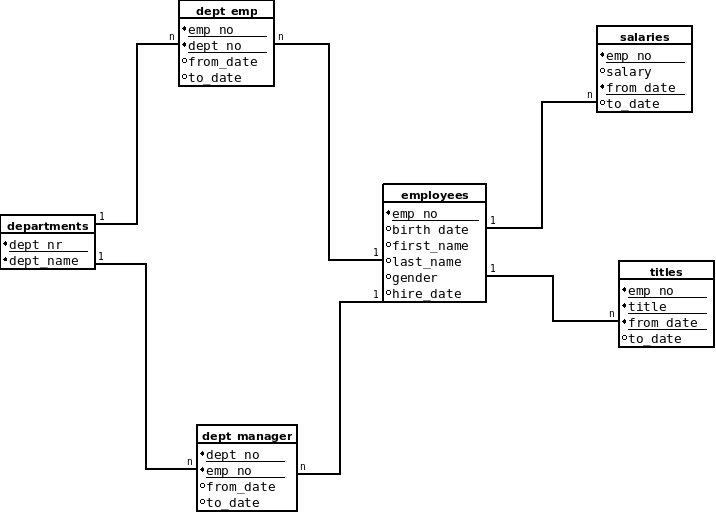
\includegraphics[width=17cm]{employees.png}


\section{Ein paar Auswertungen dazu...}

Bitte mit \texttt{RMySQL} auf die \textbf{employees}-Datenbank verbinden und folgende Darstellungen/Analysen erstellen. Die Vorgangsweise ist immer gleich wie beim gemeinsamen Beispiel zu den Abfragen:




Hinweis zur Auswertung dieser Aufgaben: Die Daten nicht zusammengefasst aus der DB holen, der Boxplot soll ja die Verteilung zeigen.

\subsection{Wie viele Personen arbeiten aktuell (YEAR(to\_date) =9999) in welchen Abteilungen? (Als Barplot dargestellt)}

\subsection{Bitte als Boxplots veranschaulichen und interpretieren:}

\subsubsection{Den aktuellen Verdienst von Frauen und Männern gegenübergestellt}

\subsubsection{Den aktuellen Verdienst in den einzelnen Abteilungen gegenübergestellt}

\subsection{Die Gehaltsentwicklung (also die einzelnen Gehälter über die Zeit - ein Mitarbeiter kann mehrere Gehaltssprünge hinter sich haben) des Mitarbeiters mit der \texttt{emp\_no 492917} als Liniendiagramm dargestellt}

Auf die Zeitsprünge, wann die einzelnen Gehaltserhöhungen stattfinden, muss keine Rücksicht genommen werden.

\subsection{Angenommen, die Gehälter wachsen linear, wie schaut dann das Durchschnittsgehalt der aktuellen Gehälter im Jahr 2020 aus?}

Hier ist eine Abfrage notwendig, die das aktuelle Gehalt nach Jahren gruppiert.

\subsubsection{Bitte grafisch darstellen}

Also die einzelnen Gehälter pro Jahr gemeinsam mit der Regressionsgeraden zeichnen lassen.

\subsubsection{Den Vorhersagewert für die Jahre 2020-2030 berechnen}

Dafür bitte den Befehl \texttt{predict} (siehe Beispiel zur Regression) verwenden.

\subsection{Gibt es einen Zusammenhang (Korrelation) zwischen Alter der Mitarbeiter und deren Gehalt?
	Bitte die entsprechenden statistischen Parameter angeben.}


Die Korrelation wird mit dem Befehl \texttt{cor.test} berechnet und ergibt einen Wert zwischen -1 und 1:

\begin{itemize}
	\item \texttt{-1}: Negative Korrelation: Wenn bei einer Variable die Werte höher sind, dann sind sie bei der zweiten Variable niedriger
	\item \texttt{0}: Kein Zusammenhang zwischen den beiden Variablen
	\item \texttt{1}: Positive Korrelation: : Wenn bei einer Variable die Werte höher sind, dann sind sie bei der zweiten Variable auch höher
\end{itemize}
 
 
\underline{Hinweise}: 


\begin{itemize}
	\item Ein Beispiel-Skript zur Datenbankverbindung und Abfrage befindet sich im Moodle
	\item Idealerweise sollten die Abfragen so gemacht werden, dass die Daten schon optimal für die Weiterverwendung in R sind
	\item Es gibt ein Datenmodell in Moodle, um einen Überblick über die \texttt{employees}-DB zu bekommen
	\item Die aktuellen Werte für Gehalt, Zugehörigkeit zu einer Abteilung, ... bekommt man immer mit dem MySQL-Befehl \texttt{YEAR(to\_date) = 9999}
	\item RMySQL holt per default nicht alle Werte, das kann man mit der Einstellung \texttt{n=-1 }abstellen:
	\begin{lstlisting}
res <- dbSendQuery(con, '<my_query>')
data1 <- fetch(res, n = -1)	
	\end{lstlisting}
\end{itemize}	
	
\end{document}